\documentclass[reprint,amsmath,amssymb,aps,]{revtex4-2}
\usepackage{graphicx}
\usepackage{dcolumn}
\usepackage{bm}
\usepackage{scrextend}
\usepackage{vmargin}
\usepackage{multirow}
\usepackage[utf8]{inputenc}
\usepackage[spanish, es-tabla]{babel}
\usepackage{enumerate}
\usepackage{float}
\usepackage{lipsum}
\usepackage{amsmath, amsthm, amssymb, amsfonts}
\usepackage[usenames]{color}
\usepackage[breaklinks=true,hidelinks]{hyperref}
\pagestyle{empty}
\spanishdecimal{.}
\begin{document}
\preprint{APS/123-QED}
\begin{abstract}
\lipsum[1]
\end{abstract}
\begin{titlepage}
\begin{center}

\includegraphics[scale=0.40]{../../../Logos/uanl.png} 
\hspace{2.5cm}

\includegraphics[scale=0.40]{../../../Logos/fcfm.png}
\end{center}
\vspace{2cm}
\begin{center}
\textbf{
UNIVERSIDAD AUTÓNOMA DE NUEVO LEÓN\\
FACULTAD DE CIENCIAS
FÍSICO MATEMÁTICAS}\\
\vspace*{2cm}
\begin{large}
\vspace{1cm}
\large{\textbf{Aplicaciones de la Mecánica Cuántica}}\vspace{1.5cm}\\
\textbf{Tarea 2:\\ Indexación de un patrón de \\difracción de electrones}\\
Carlos Luna\\
\end{large}
\vspace{3.5cm}
\begin{minipage}{0.6\linewidth}
\vspace{0.5cm}
\changefontsizes{14pt}
Nombre:\\
Giovanni Gamaliel López Padilla\\
\end{minipage}
\begin{minipage}{0.2\linewidth}
\changefontsizes{14pt}
Matricula:\\
1837522\\
\end{minipage}
\end{center}
\vspace{4cm}
\begin{flushright}
\today
\end{flushright}
\pagebreak
\end{titlepage}
\maketitle
\section{Introducción}
\section{Objetivo}
Realizar una indexación a un sistema de átomos de plata dado sus parámetros de difracción de electrones.
\section{Marco teórico}
La difracción de electrones se basa en la teoría cuantica de la dualidad onda-partícula. El haz de electrones se comporta como un conjunto
de ondas que inciden sobre el material cristalino y se difractam en los centros de dispersión, lugares donde la densidad electrónica es más alta
esto quiere decir que en esa posición es más probable de encontrar a los átomos que conforman el material.\\ 
La difracción de electrones es una técnica muy utilizada en Física de Materiales. La estructura periódica
de un sólido cristalino actúa como una red de difracción para los electrones, pues la longitud de onda de
los electrones tiene un tamaño parecido al espaciado interatómico. Esto lo convierte en una buena
alternativa a la difracción de rayos X para
estudiar la estructura cristalina de los
materiales. En cada caso, los electrones cumplen una relación de interferencia constructiva distinta, aunque todos
ellos son muy similares a la relación del ejercicio (donde, por simplicidad, en lugar de un material, se
trata una cadena monoatómica con distancia interatómica similar al parámetro de red del Si) y se
obtienen de la misma forma: a partir de imponer que la diferencia de caminos entre los haces
difractados sea igual a un número entero de longitudes de onda. Se pueden sacar conclusiones del
ejercicio válidas para todos los casos: los patrones son simétricos en torno a $\theta$=0 y $sin(\theta)$ es
inversamente proporcional al parámetro de red a y proporcional a la raíz cuadrada de la energía de los
electrones incidentes.\\
Para este caso tenemos un material de plata, este material cristalino cumple con los parámetros 
mostrados en la tabla \ref{tabla:parametros}.
\begin{table}[H]
    \centering
    \begin{tabular}{ccccc}\hline
        2$\theta$ & Intensity & D-Spacing (\r{A}) & HKL & Multiplicity\\ \hline
        38.15 & 100 & 2.3592 & 111 & 8 \\
        44.34 & 46.77 & 2.0431 & 200 & 6 \\
        66.50 & 25.61 & 1.447 & 220 & 12 \\
        77.47 & 27.18 & 1.2320 & 311 & 24 \\
        81.62 & 7.69 & 1.1796 & 222 & 8 \\ \hline
    \end{tabular}
    \caption{Parámetros para el sistema de plata con densidad $\rho=10.500 g/cm^{3}$, irradiado con un haz de $1.541838$\r{A}}
    \label{tabla:parametros}
\end{table}
La Configuración de posiciones de los átomos de plata en nuestro material cristalino son los mostrados en la figura \ref{fig:inicial}.
\begin{figure}[H]
    \centering
    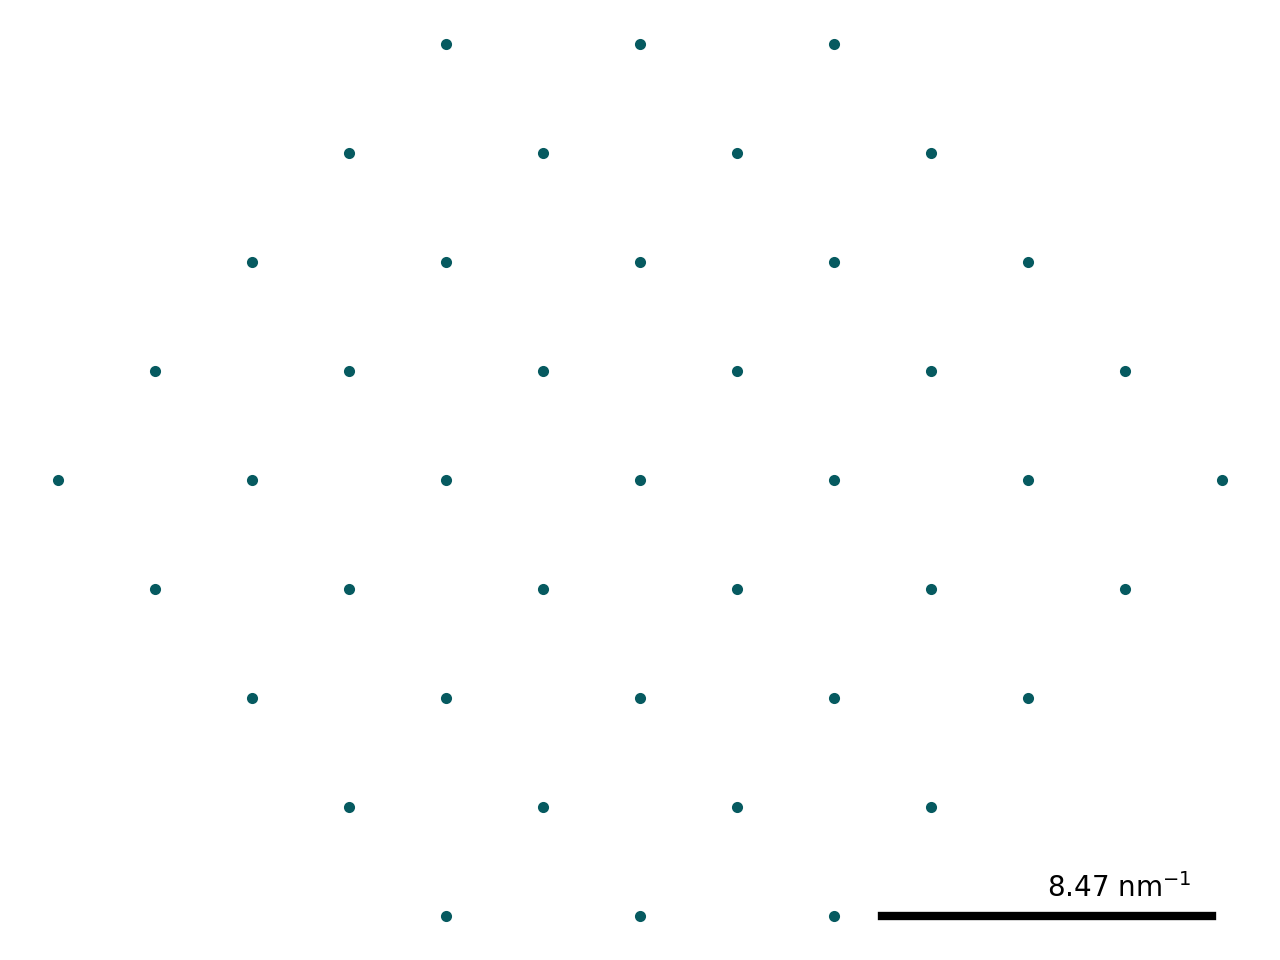
\includegraphics[scale=0.4]{../Graphics/inicial.png}
    \caption{Configuración de los átomos de Plata}
    \label{fig:inicial}
\end{figure}
Para poder identificar que distancias interatomicas son importante para el estudio se propusieron las siguientes condiciones:\\
Dado un punto de referencia llamado centro u órigen y dos puntos i,j tal que $i\neq j$  se tiene que cumplir que:
\begin{enumerate}
    \item La distancia entre el centro e i, tiene que ser la misma entre el centro y j.
    \item La pendiente de los putnos del centro e i y el centro y j tiene que ser iguales.
\end{enumerate}
\section{Resultados}
Para el caso mostrado, en la figura \ref{fig:inicial}, se propuso como átomo de origen el que se encuentra en la parte central, por lo que
desarrollando un algoritmo lea las posiciones de todos los átomos e imprima las distancias interatomicas en una gráfica para observar sus relaciones,
la figura generada es la figura \ref{fig:distancias}.
\begin{figure}[H]
    \centering
    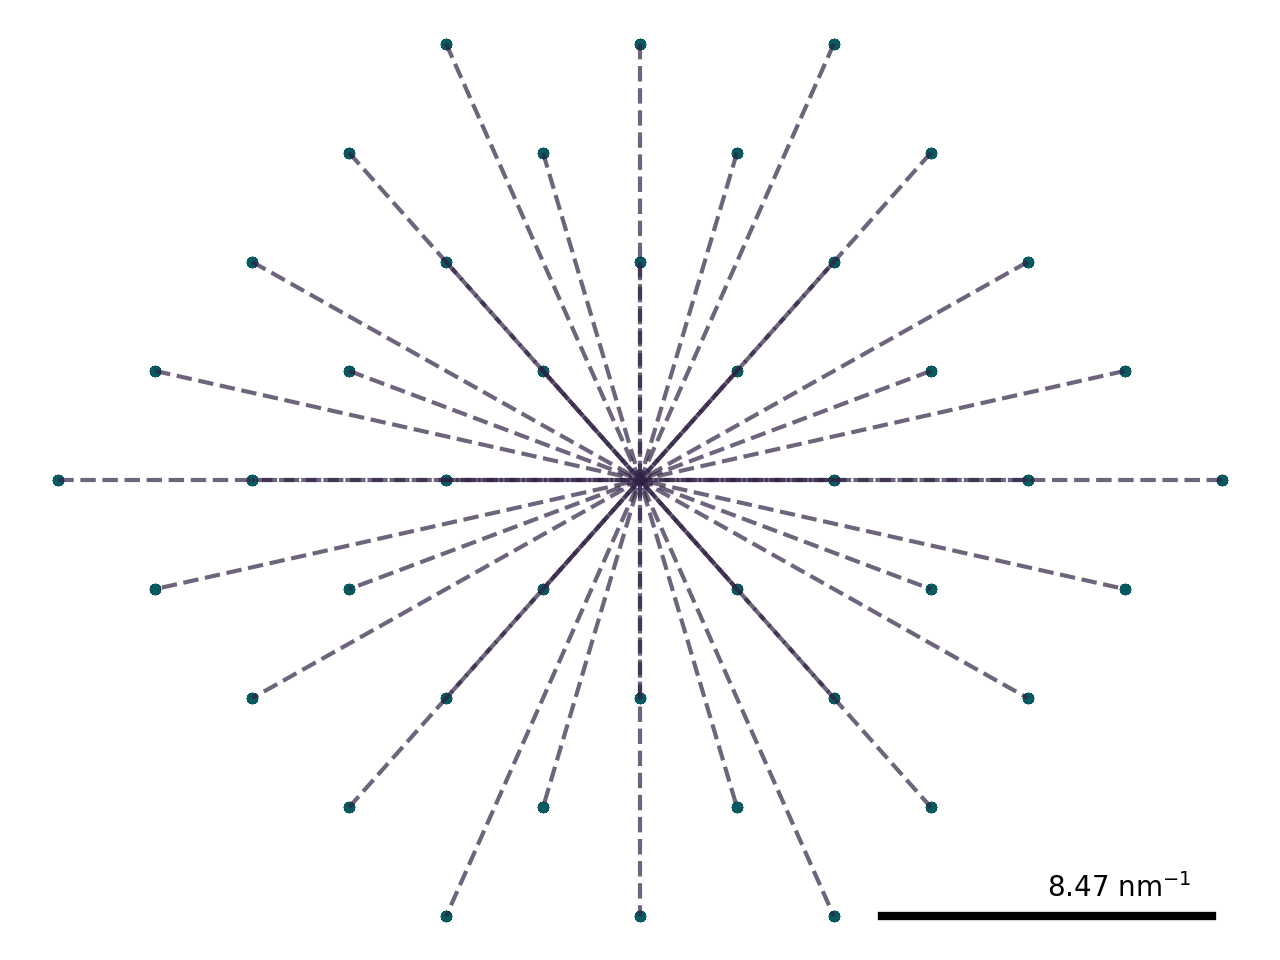
\includegraphics[scale=0.4]{../Graphics/distancia.png}
    \caption{Distancias interatomicas calculadas usando las condiciones entre tres puntos.}
    \label{fig:distancias}
\end{figure}
A la par el algoritmo calcula las distancias interatomicas que cumplan las condiciones, con ello realiza una relación con los parámetros mostrados en la tabla \ref{tabla:parametros},
llegando así a encontrar las familias de los indices de Miller para todos los átomos de plata, estos indices estan mostrados en la 
figura \ref{fig:indicesmiller}.
\begin{figure}[H]
    \centering
    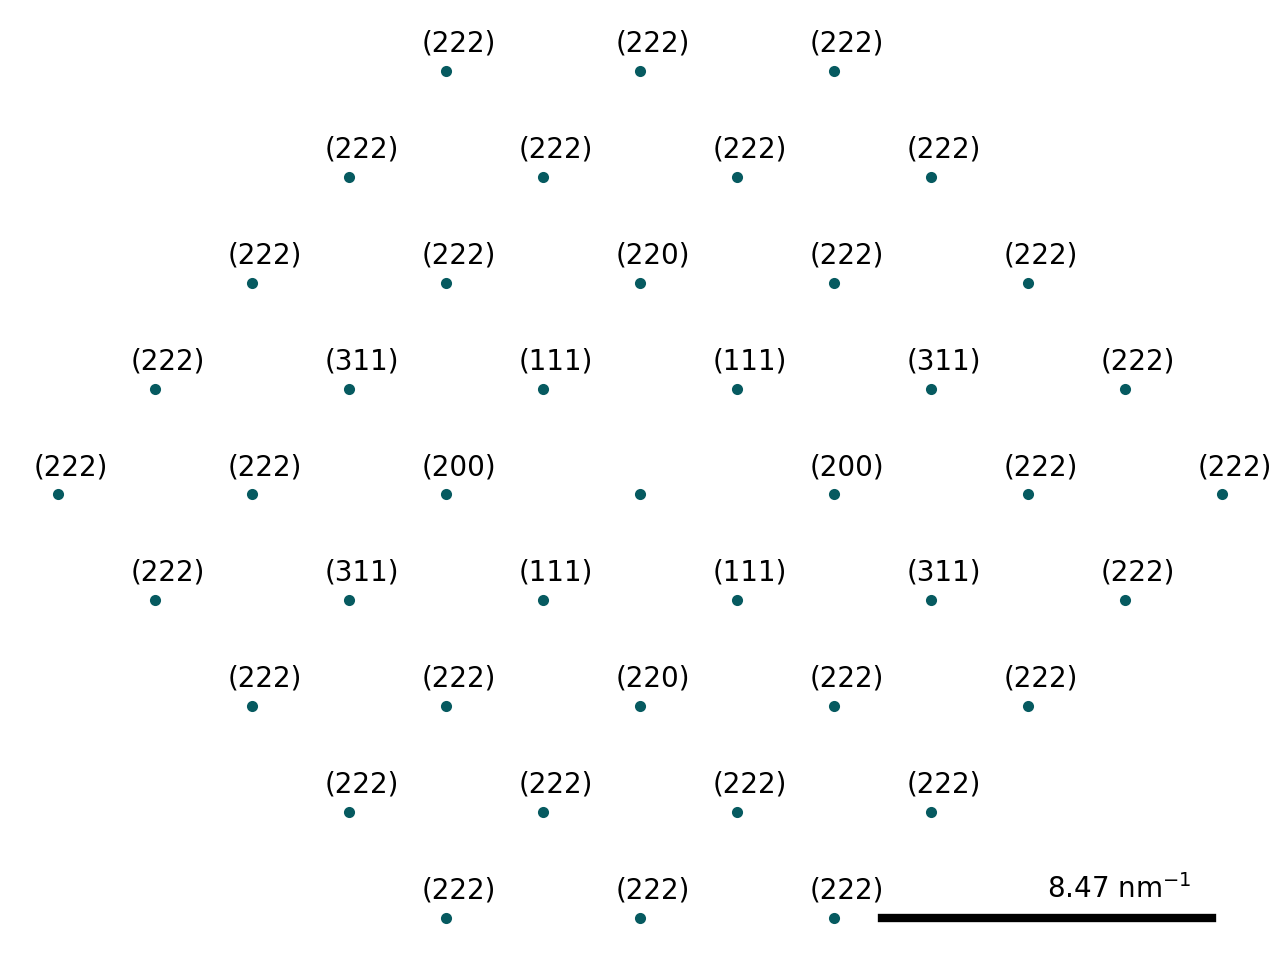
\includegraphics[scale=0.4]{../Graphics/indices.png}
    \caption{Familia de indices de Miller asignados a partir de los datos de la tabla \ref{tabla:parametros} usando el código \ref{cod:distancias}}
    \label{fig:indicesmiller}
\end{figure}
Tomando a los átomos con la familia de (111), se propusieron indices de Miller de forma en que fueran diferentes y a partir de esto se calcularon 
los demás indices. Estos indices de Miller estan mostrados en al figura \ref{fig:lattice}
\begin{figure}[H]
    \centering
    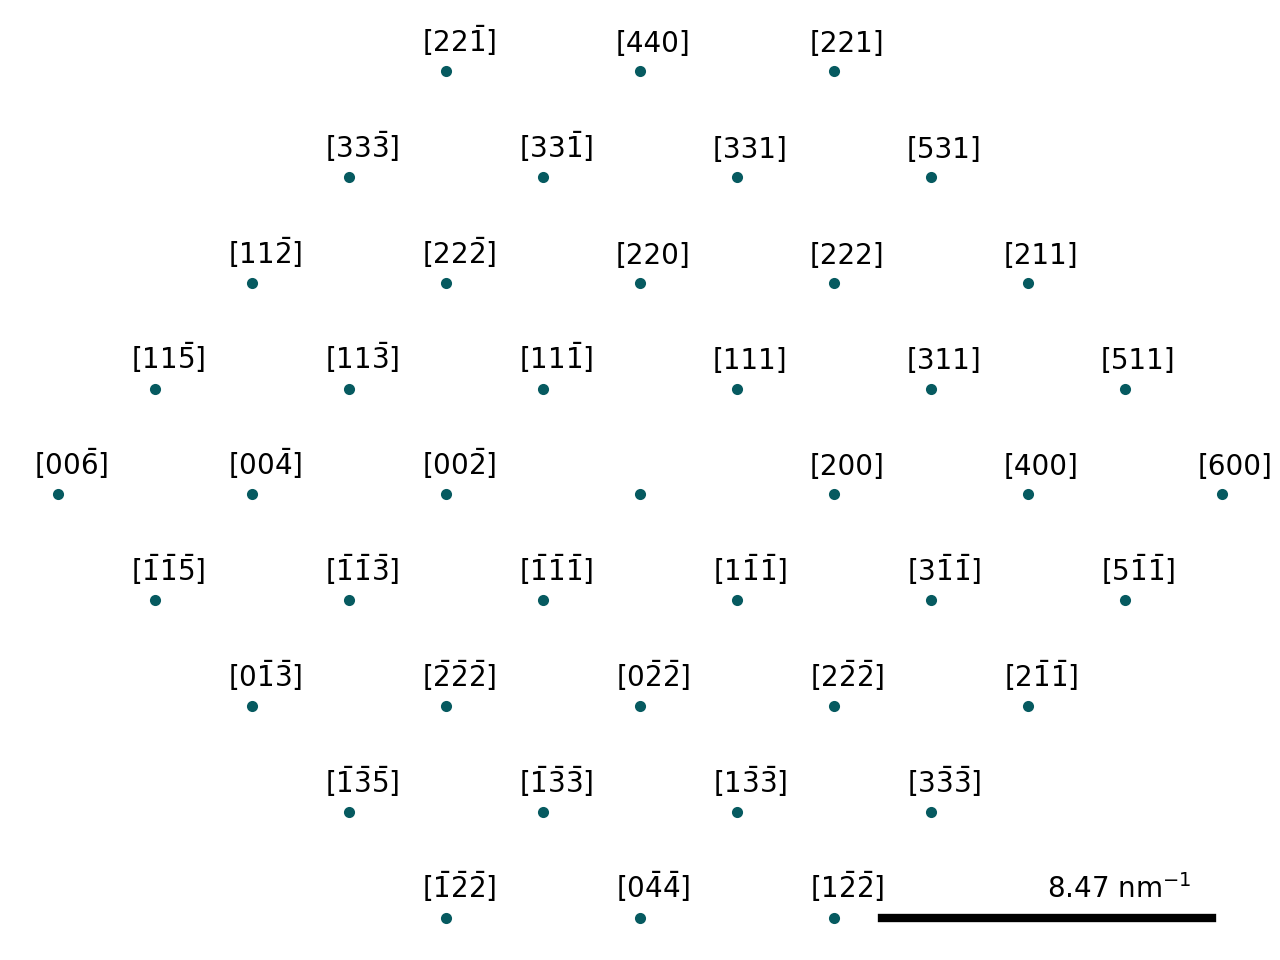
\includegraphics[scale=0.4]{../Graphics/lattice.png}
    \caption{Indices de Miller asignados a partir de la suma vectorial con los indices de la familia (111) como valores iniciales.}
    \label{fig:lattice}
\end{figure}
\section{Conclusiones}
\section{Código}
\begin{enumerate}
    \item \href{https://github.com/giovannilopez9808/Notas_Agosto_2020/blob/master/AMC/Tarea2/distancia.py}{Distancia.py\label{cod:distancias}}\\
    Este código realiza las figuras \ref{fig:inicial}, \ref{fig:distancias} y \ref{fig:indicesmiller} a partir de la posición de los átomos y la información de la tabla \ref{tabla:parametros}
\end{enumerate}
\bibliographystyle{plain}
\nocite{*}
\bibliography{Main}
\end{document}